\documentclass[12pt, titlepage]{article}

\usepackage[section]{placeins}
\usepackage{enumerate}
\usepackage{booktabs}
\usepackage{tabularx}
\usepackage{hyperref}
\usepackage{graphicx}
\usepackage{float}
\usepackage{attachfile}
\usepackage{ulem}

\hypersetup{
    colorlinks,
    citecolor=black,
    filecolor=black,
    linkcolor=red,
    urlcolor=blue
}
\usepackage[round]{natbib}

\title{SE 3XA3: Software Requirements Specification\\TankWar}

\author{Team \#212, Genius
		\\Di Wu, 400117248, wud43 
		\\Jiahao Zhou, 400082351, zhouj56 
		\\Xinyu Huang, 400120376, huangx65
}

\date{\today}


\begin{document}

\maketitle

\pagenumbering{roman}
\tableofcontents
\listoftables
\listoffigures

\begin{table}[bp]
\caption{\bf Revision History}
\begin{tabularx}{\textwidth}{p{3cm}p{2cm}X}
\toprule {\bf Date} & {\bf Version} & {\bf Notes}\\
\midrule
Feb. 2, 2020 & 1.0 & Creates the first version of SRS\\
\textcolor{red}{Feb. 26, 2020} & \textcolor{red}{2.0} & \textcolor{red}{Follows all the comments from TA to improve the SRS. Fixed some of the minor issues. Improve the functional and nonfucntional requirements. Makes the document consistent.}\\
\textcolor{red}{April. 2, 2020} & \textcolor{red}{2.1} & \textcolor{red}{The rationales behind the functional requirements are added into the SRS. Fixed some minor issues.}\\
\bottomrule
\end{tabularx}
\end{table}

\newpage

\pagenumbering{arabic}

This document describes the requirements for TankWar. The template for the Software
Requirements Specification (SRS) is a subset of the Volere template~\citep{RobertsonAndRobertson2012}.  %If you make further modifications
%to the template, you should explicity state what modifications were made.

\section{Project Drivers}

\subsection{The Purpose of the Project}
The purpose of this \underline{project} is to recreate and upgrade the game BattleCity. BattleCity was one of the most popular games decades ago, and it was usually on family computers. However, a family computer is hard to find today, and the game BattleCity is also someway too simple for today’s person, so we are going to upgrade it to a new game called TankWar, which will be compatible with modern computers. Also more modes will be added in the upgraded version. The first one is the player versus player mode, which can increase the competitiveness of the game. The other new mode is the map editor, which allows the players to create a new map on their own to increase their interest.
\subsection{The Stakeholders}

\subsubsection{The Client}
The clients for this \underline{project} are Dr.Asghar A Bokhari, and the TAs, Andrew Lucentini and Maryam Hosseinkord. They will be the final reviewer of our \underline{project}.
\subsubsection{The Users} 
The users for this \underline{project} are all the people who want to play this new game. \textcolor{red}{Therefore, the potential users can be anyone above 12 years old with simple compute operation knowledge and the ability to operate a keyboard.} \textcolor{red}{\sout{Our game is developed for all ages. Therefore the potential costumers can be anyone at any age.}}\\

\textcolor{red}{Comments: This was "The Customers" in the original template, but I think the word users are more appropriate since our product is totally free and accessible for anyone.}

\subsubsection{Other Stakeholders}
The other stakeholders are the \underline{developers}, who are the three team members in our group. Redeveloping the whole program and implementing new functions will be developers' responsibilities.
\subsection{Mandated Constraints}
\begin{enumerate}[1.]
	\item The \underline{project} must be finished in one term, by April 6, 2020.
	\item The new game should be able to run under Windows system \textcolor{red}{that later than Windows 7}, Mac OS X \textcolor{red}{10.0} system, and Linux \textcolor{red}{Ubuntu 18.0} system with python and pygame. 
	\item The new game will be free and accessible for all the players.  
	
\end{enumerate}

\subsection{Naming Conventions and Terminology}
\begin{enumerate}[1.]
	\item \textbf{Developers}: The team members.
	\item \textbf{Project}: TankWar project. Recreate and upgrade the original game BattleCity.
	\item \textbf{\textcolor{red}{\sout{User}}} \textcolor{red}{\sout{: The players of the TankWar game.}}
	\item \textbf{PVE}: Player1 and Player2 Versus Environment.
	\item \textbf{PVP}: Player1 Versus Player2.
\end{enumerate}

\subsection{Relevant Facts and Assumptions}
\subsubsection{Relevant Facts}
\begin{itemize}

\item In the original TankWar game(BattleCity), there are 1012 lines of code.
\item The original game is written in python.
\end{itemize}
 

\subsubsection{Assumptions}
\begin{itemize}
 
\item Python and pygame are assumed already being installed on the \underline{users}' computer.
\item The game is assumed to be played by two players.
\item \textcolor{red}{A US standard keyboard is assumed to be available for the players.}
\item \textcolor{red}{The players are assumed to be able to operate a keyboard.}
\item \textcolor{red}{The players are assumed to have simple computer operation knowledge.}
\item \textcolor{red}{The users' computer are assumed to meet the minimum requirements for 2-cores processor and 1GB RAM.}
\end{itemize}
 

\section{Functional Requirements}

\subsection{The Scope of the Work and the Product}
\subsubsection{The Context of the Work}
\newpage
\begin{figure}[H]
  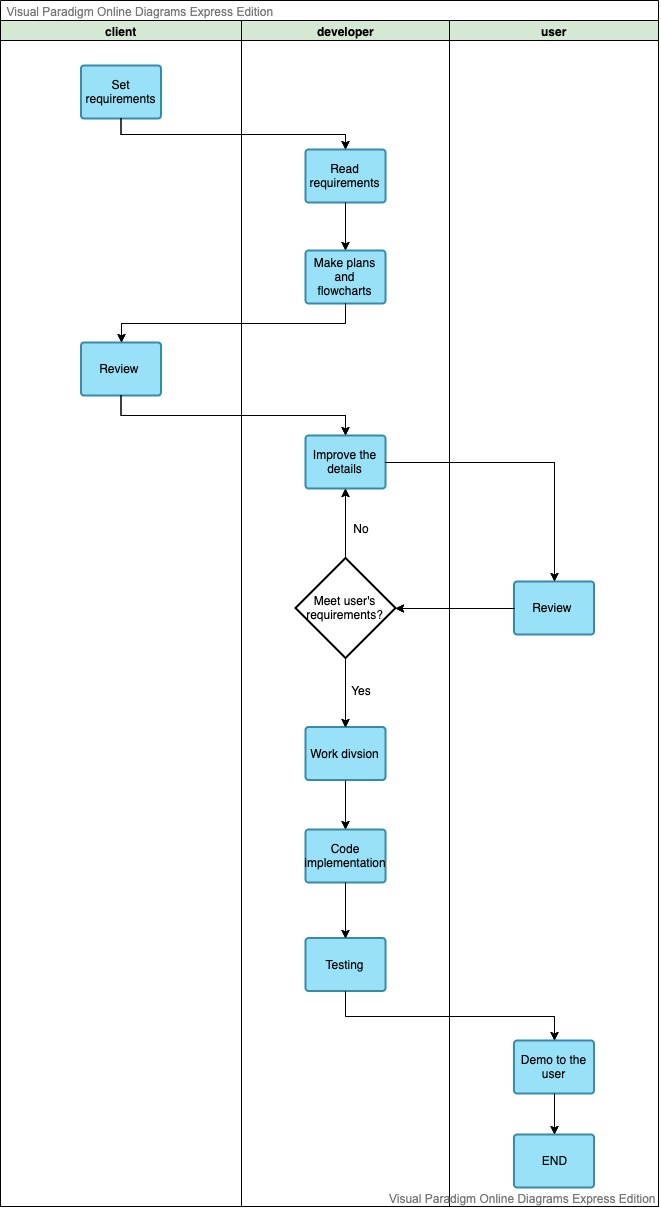
\includegraphics[width=0.75\linewidth]{SL.jpg}
  \caption{Swimlane Diagram.}
  \label{fig:Swimlane Diagram}
\end{figure}

\subsubsection{\textcolor{red}{Work Partitioning}}
\begin{table}[H]
\begin{tabular}{|p{3cm}|p{3cm}|p{3cm}|p{3cm}|}
 \hline
 Event Number & Event Name & Input & Output\\ 
 \hline
 1 & TankWar Game Interface Creation& Python Code & User Interface\\ 
 \hline
 2 & Map Editor & Python Codes, graphics, and user's operations & A created map file \\ 
 \hline
 3 & Tank Control & Python Codes and user's operation & Movements and attack of the tank. \\
 \hline
 4 & Tank Object & Python Code & Characteristics and the corresponding ultimate skill will be determined.\\
 \hline
 5 & \underline{PVP} and \underline{PVE} mode & Python Code & Rules of \underline{PVP} and \underline{PVE} mode will be implemented.\\
  \hline
 6 & Game result determination & Python Code & Game status will be able to detected and a end screen will be shown.\\
  \hline
\end{tabular}
\caption{Work Partitioning Table}
\label{table:Work Partitioning Table}
\end{table}

\subsubsection{Individual Product Use Cases}
\newpage
\begin{figure}[H]
  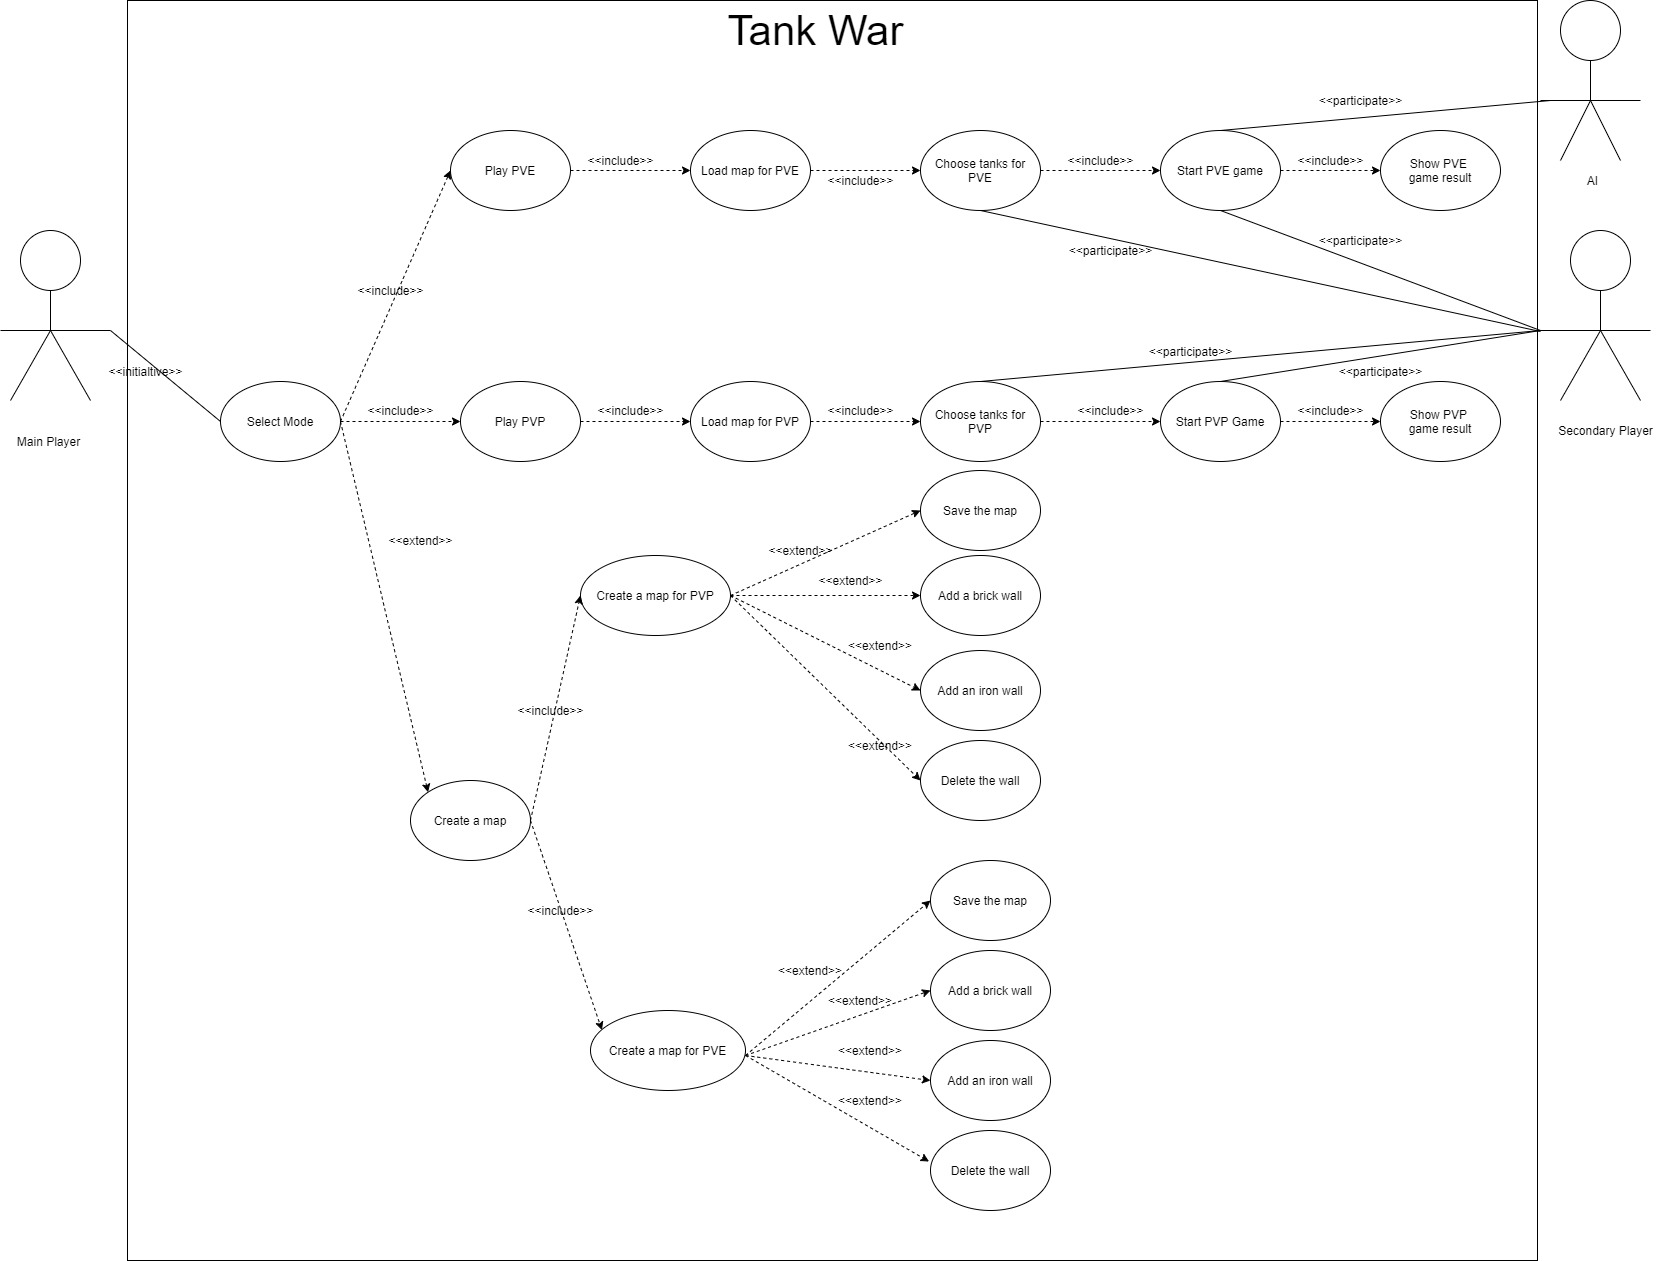
\includegraphics[width=1.4\linewidth, angle =270]{UC.jpg}
  \caption{Use Case Diagram.}
  \label{fig:use case1}
\end{figure}

\begin{figure}[H]
  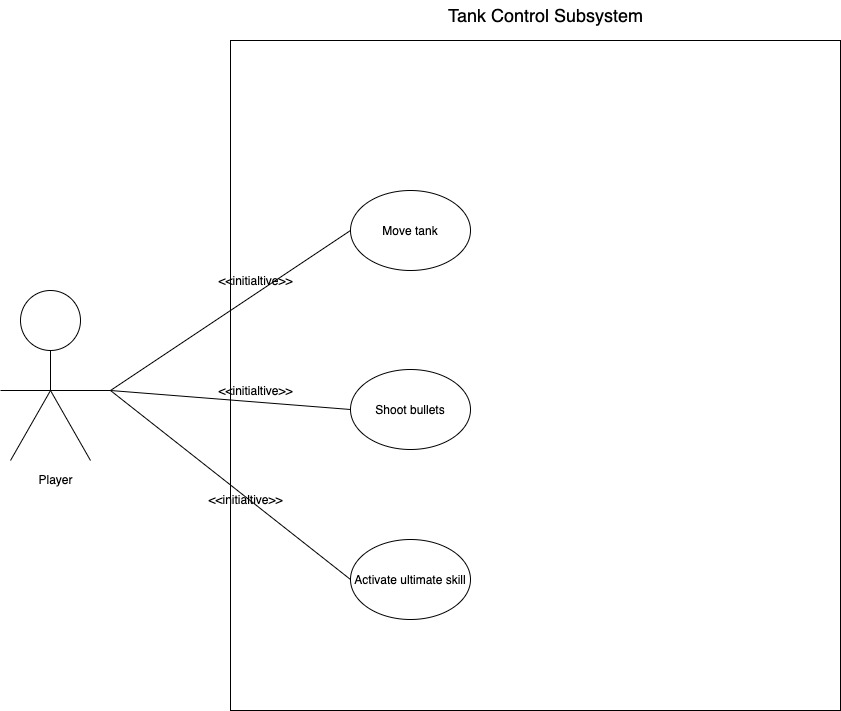
\includegraphics[width=0.9\linewidth]{TC.jpg}
  \caption{Tank Control Use Case Diagram.}
  \label{fig:tank control use case2}
\end{figure}

\textcolor{red}{Comments: There are two players in either the \underline{PVE} or \underline{PVP}. Only the rules of the the two game mode is different. The player 2 is involved in \underline{PVE} mode to control the second tank and fight side by side with the player 1's tank.}

\begin{itemize}

\item \textbf{Select mode}: Player shall be able to select mode.
\item \textbf{Play \underline{PVE}}: Player selects player-versus-environment mode.
\item \textbf{Play \underline{PVP}}: Player selects player-versus-player mode.
\item \textbf{Create a map}: The map is created in the map-editing mode.
\item \textbf{Create a map for PVE}: The map for PVE mode is created.
\item \textbf{Create a map for PVP}: The map for PVP mode is created.
\item \textbf{Save the map}: Once created, the map is saved on the computer.
\item \textbf{Add a brick wall}: Add a brick wall on the map creating right now.
\item \textbf{Add a iron wall}: Add a iron wall on the map creating right now.
\item \textbf{Delete a wall}: Delete a wall from the map.
\item \textbf{Load map for \underline{PVE}}: Load a map for the \underline{PVE} game.
\item \textbf{Load map for \underline{PVP}}: Load a map for the \underline{PVP} game.
\item \textbf{Choose tanks for \underline{PVE}}: Players choose the tank before the \underline{PVE} game starts.
\item \textbf{Choose tanks for \underline{PVP}}: Players choose the tank before the \underline{PVP} game starts.
\item \textbf{Start \underline{PVE} game}: \underline{PVE} game starts.
\item \textbf{Start \underline{PVP} game}: \underline{PVP} game starts.
\item \textbf{Show \underline{PVP} game result}: Game result of \underline{PVP} mode is display on the screen.
\item \textbf{Show \underline{PVE} game result}: Game result of \underline{PVE} mode is display on the screen.
\item \textbf{Move tank}: Player moves the tank.
\item \textbf{Shoot bullets}: Player shoots the bullets.
\item \textbf{Activate ultimate skills}: Player activates the ultimate skill of the tank.



\end{itemize}
\subsection{Functional Requirements}

  FR1. The system shall provide three mode to the users including "Player vs. Environment", "Player 1 vs. Player 2", and "Map Editing" at the beginning of the system.\\
  \textcolor{red}{Rationale: There should be three modes in our game. And all the three modes should be shown to the users.\\
  Fit criterion: After opening the game, check whether there is a screen for selecting the modes.}\\ \newline
  FR2. The system shall allow the users to add brick walls, add iron walls, and delete walls in the map editing mode.\\
  \textcolor{red}{Rationale: These are the main functions in map editing mode. Users can only created their own maps by using these functions.\\
  Fit criterion: After selecting the map editing mode, check whether there is brick wall or iron wall shown after pressing "J" key or "K" key.}\\ \newline
  FR3. The system must allow the users to save and load the map they created in map editing mode.\\ 
  \textcolor{red}{Rationale: The users should be allowed to save their map so that it can be opened during the gaming.\\
  Fit criterion: Check whether there is the corresponding file in the local computer after saving the map. Check whether the corresponding file can be loaded during the game.}\\ \newline
  FR4. \textcolor{red}{\sout{The system shall include the function of moving the tank to four different directions: forward, back, left, and right.}}
  The system shall include the function of moving the tank to four different directions: forward, back, left, and right using arrow keys or "WASD" keys on the keyboard.\\
  \textcolor{red}{Rationale: With this functional requirement, the users can move the tank.\\
  Fit criterion: After entering the game, check whether player 1 and player 2 can move the tank by pressing "WASD" keys and arrow keys.}\\ \newline
  FR5. The system shall allow the player 1 and player 2 to use the ultimate skill of the selected tank by pressing "K" and "." keys on keyboard respectively.\\
  \textcolor{red}{Rationale: Users should be able to use the ultimate skills.\\
  Fit criterion: After entering the game, check whether player 1 and player 2 can use the ultimate skill by pressing "K" and "." keys.}\\ \newline
  FR6. \textcolor{red}{\sout{The system shall allow the users to shoot the bullet while controlling the tank.}} The system shall allow the player 1 and player 2 to shoot the bullet while controlling the tank using "J" and "," keys on the keyboard respectively.\\
  \textcolor{red}{Rationale: Users should be able to shoot in order to kill enemy or kill each other.\\
  Fit criterion: After entering the game, check whether player 1 and player 2 can shoot by pressing "J" and "," keys.}\\ \newline
  FR7. \textcolor{red}{\sout{The system shall allow the bullets to destroy the brick walls.}} The system shall allow the bullets to destroy the brick walls when the bullets hit the brick wall.\\
  \textcolor{red}{Rationale: The brick wall should be destroyed by bullets. \\
  Fit criterion: After entering the game, check whether the brick wall can be destroyed after a bullet hitting the brick wall.}\\ \newline
  FR8. The system shall not allow the bullets to destroy the iron walls when the bullets hit the iron wall.\\
  \textcolor{red}{Rationale: The iron wall should not be destroyed by bullets. \\
  Fit criterion: After entering the game, check whether the iron wall can be destroyed after a bullet hitting the iron wall.}\\ \newline
  FR9. The walls shall block the movements of the tanks.\\
  \textcolor{red}{Rationale: The tank should not be allowed to walk over the walls.\\
  Fit criterion: After entering the game, check whether the tank can move pass the wall while facing the wall and "W" or up arrow key is pressed and held.}\\ \newline
  FR10. The system shall allow the users to choose one among three different kinds of tanks before the game starts in both \underline{PVE} and \underline{PVP} mode which includes double-life tank, high-speed tank, double-bullet tank.\\
  \textcolor{red}{Rationale: The users should be able to choose the tank based on their preference.\\
  Fit criterion: After entering the game, check whether there is a screen of tank selection.}\\ \newline
  FR11. The system shall display the result of the game after the game ends including winning, losing, and draw.\\
  \textcolor{red}{Rationale: The game should notify the users about the result.\\
  Fit criterion: After finishing the game, check whether there is a result screen.}\\ \newline
  FR12. The game shall offer different buffs in the map after the game starts, including moving speed enhanced buff, wall enhanced buff, and bullet speed enhanced buff.\\
  \textcolor{red}{Rationale: Buffs should be provided in the game to make the game more fun.\\
  Fit criterion: After entering the game, check whether the system generates buffs and show them on the map.}\\ \newline
  FR13. \textcolor{red}{\sout{The system shall provide enemy tanks in PVE mode.}} The system shall provide enemy tanks in \underline{PVE} mode and make them move automatically so that the player can distinguish.\\
  \textcolor{red}{Rationale: The moving ability of enemy tanks is very important in PVE mode.\\
  Fit criterion: After entering the game, check whether the enemy tanks can move by themselves.} \\ \newline
  FR14. The system shall control enemy tanks and shoot the bullet to fight against the players' tanks in \underline{PVE} mode.\\
  \textcolor{red}{Rationale: The shooting ability of enemy tanks is very important in PVE mode.\\
  Fit criterion: After entering the game, check whether the enemy tanks can shoot by themselves.} \\ \newline
  FR15. The system shall allow the enemy tanks to relive immediately after they \textcolor{red}{are destroyed in the \underline{PVE} mode.\\
  Rationale: Enemy tanks need to be able to relive to keep the PVE game process continuous.\\
  Fit criterion: After entering the game, check whether the enemy tanks can relive after being destroyed.}\\ \newline
  FR16. The number of enemy tanks on the battle field in \underline{PVE} mode shall be five at all time.\\
  \textcolor{red}{Rationale: The number of enemy tanks should be controlled. \\
  Fit criterion: After entering the game, check whether the number of enemy tanks is equal to 5.}\\ \newline
  FR17. The system shall provide a home base for players in \underline{PVE} mode.\\
  \textcolor{red}{Rationale: Home base is one of the main element for determining the game result.\\
  Fit criterion: After entering the game, check whether home base is provided.}\\ \newline
  FR18. The system shall provide two home bases for players in \underline{PVP} mode.\\
  \textcolor{red}{Rationale: Home bases are main elements for determining the game result.\\
  Fit criterion: After entering the game, check whether home bases are provided.}\\ \newline
  FR19. In \underline{PVE} mode, the system shall display the lost result if the players' home base is destroyed or the players' tanks died 3 times in 3 minutes, otherwise display the win result.\\
  \textcolor{red}{Rationale: The rules of PVE mode are necessary for PVE game.\\
  Fit criterion: Check whether the corresponding result is shown after finishing the whole game. To be more specific, check whether the win result is showned if both players' tanks did not die for three times or the home base is destroyed. Check whether the lost result is showned after both players' tanks is destroyed three times or the home base is destrroyed.}\\ \newline
  FR20. In \underline{PVP} mode, the system shall display a win result if the player's tank destroy another player's home base or kill the other player's tank 3 times in 3 minutes. Otherwise it will be a tie.\\
  \textcolor{red}{Rationale: The rules of PVP mode are necessary for PVP game.\\
  Fit criterion: Check whether the tie result is shown if no home base is destroyed or no player's tank is destroyed three times in 3 minutes. Check whether the player 1 win result is shown if player 1's tank destroys player 2's tank three times or destroys player 2's home base in 3 minutes. Check whether the player 2 win result is shown if player 2's tank destroys player 1's tank three times or destroys player 1's home base in 3 minutes.}\\ \newline 
  FR21. All the players' tanks in both \underline{PVP} and \underline{PVE} mode shall have only 3 life.\\
  \textcolor{red}{Rationale: Both player's tanks only have 3 life because it is a element for determining the result of the game.\\
  Fit criterion: After entering the game, check whether the tank can still relive after being destroyed three times.}\\ \newline
  

\section{Non-functional Requirements}

\subsection{Look and Feel Requirements}

\subsubsection{Appearance Requirements}
\label{ssub:appearance_requirements}
% Begin SubSubSection
\begin{enumerate}[{LF}1. ]
	\item The TankWar shall be designed as a 2-D game.
	\\
	
	Fit Criterion: The TankWar game and system are in 2 dimension.
\end{enumerate}
% End SubSubSection

% Begin SubSubSection
\begin{enumerate}[{LF}2. ]
	\item The background of the TankWar system shall be black.
	\\
	
	Fit Criterion: The background is black.
\end{enumerate}
% End SubSubSection

% Begin SubSubSection
\begin{enumerate}[{LF}3. ]
	\item The brick walls and iron walls shall be arranged in a grid map. 
	\\
	
	Fit Criterion: The system displays brick walls and iron walls in a grid map. 
\end{enumerate}
% End SubSubSection

% Begin SubSubSection
\begin{enumerate}[{LF}4. ]
	\item Brick walls shall look like bricks and their colour shall be orange.
	\\
	
	Fit Criterion: The brick walls are orange like bricks. 
\end{enumerate}
% End SubSubSection

% Begin SubSubSection
\begin{enumerate}[{LF}5. ]
	\item An iron wall shall consist of 4 iron cube and their colour shall be sliver.
	\\
	
	Fit Criterion: The iron walls are sliver and one iron wall has 4 small iron cube.
\end{enumerate}
% End SubSubSection

% Begin SubSubSection
\begin{enumerate}[{LF}6. ]
	\item Different types of the tanks in the TankWar system shall be used different colour to represent.
	\\
	
	Fit Criterion: The system shall display different types of tanks with different colour.
\end{enumerate}
% End SubSubSection

% Begin SubSubSection
\begin{enumerate}[{LF}7. ]
	\item The icon of the home in TankWar system shall look like a\textcolor{red}{n} eagle.
	\\
	
	Fit Criterion: The system shall display a home which looks like a eagle.
\end{enumerate}
% End SubSubSection

\subsubsection{Style Requirements}
\label{ssub:style_requirements}
% Begin SubSubSection
\begin{enumerate}[{LF}8. ]
	\item The TankWar system shall follow the drawing style of the original game "Battle City".
	\\
	
	Fit Criterion: \textcolor{red}{By surveying 50 test users, 80 percent of the test users consider the drawing style of TankWall shall be more than 90 percent similar with Battle City. \sout{By comparing the original game ”Battle City” with TankWar, the drawing style of TankWall shall be more than 90 percent similar with Battle City.}}

\end{enumerate}
% End SubSubSection

\subsection{Usability and Humanity Requirements}
\label{sub:usability_and_humanity_requirements}
% Begin SubSection

\subsubsection{Ease of Use Requirements}
\label{ssub:ease_of_use_requirements}
% Begin SubSubSection
\begin{enumerate}[{UH}1. ]
	\item The system shall provide the photos and descriptions of different types of tanks to give a brief introduction when users are choosing tanks at the beginning of the game.
	\\
	
	Fit Criterion: The photos and descriptions are displayed on the screen when users are choosing tanks at the beginning of the game.
\end{enumerate}
% End SubSubSection

\begin{enumerate}[{UH}2. ]
	\item The system shall display the rules of the game for 3 seconds before starting the game.
	\\
	
	Fit Criterion: The rules of the game are displayed for 3 seconds before starting the game.
\end{enumerate}
% End SubSubSection

\begin{enumerate}[\textcolor{red}{\sout{{UH}3}}. ]
	\item \textcolor{red}{\sout{The player's tank in the game shall be controlled by 4 direction keys and two functional keys. The direction keys shall use "wasd" and "up down left right" for each player. The function keys shall use the key "j" and "." as the shoot key, while the key "k" and "?" shall be used to activate the ultimate skills of the tanks.}} 
	\\
	
	\textcolor{red}{\sout{Fit Criterion: The tanks can be used "wasd" and "up down left right" to control the movements, while shooting function is activated by "j" and "." and clicking "k" and "?" can activate the ultimate skills of the tanks.}}
	
\end{enumerate}
% End SubSubSection

\begin{enumerate}[\textcolor{red}{\sout{{UH}4}}. ]
	\item \textcolor{red}{\sout{ The system shall use the buff icons that have the symbolic meaning as same as the function of the buffs to represent a buff.}}
	\\
	
	\textcolor{red}{\sout{Fit Criterion: By surveying 50 test \underline{users}, 80 percent of the test \underline{users} consider the icons are relative to the buff function.}}
\end{enumerate}

\subsubsection{Personalization and Internationalization Requirements}
\label{ssub:personalization_and_internationalization_requirements}
% Begin SubSubSection
\begin{enumerate}[\textcolor{red}{\sout{{UH}5} {UH}3}. ]
	\item Not Applicable
\end{enumerate}
% End SubSubSection

\subsubsection{Learning Requirements}
\label{ssub:learning_requirements}
% Begin SubSubSection
\begin{enumerate}[\textcolor{red}{\sout{{UH}6} {UH}4}. ]
	\item The system shall display the instruction of the game about basic rules and operations in the game before starting a battle. After reading the instruction, the user shall have basic knowledge about how to play the game.
	\\
	
	Fit Criterion: The rules and operation instruction are displayed on the screen before starting a battle. By surveying 50 test users, 80 percent of the test users knows how to play the game.
\end{enumerate}
% End SubSubSection

\subsubsection{Understandability and Politeness Requirements}
\label{ssub:understandability_and_politeness_requirements}
% Begin SubSubSection
\begin{enumerate}[\textcolor{red}{\sout{{UH}7} {UH}5}. ]
	\item The system shall use words and icons which are easily understandable by common users who are above 12 years old.
	\\
	
	Fit Criterion: By surveying 50 test users above 12 years old, 80 percent of the test users consider that the words and icons in the product are easily understandable.
\end{enumerate}
% End SubSubSection

\subsubsection{Accessibility Requirements}
\label{ssub:accessibility_requirements}
% Begin SubSubSection
\begin{enumerate}[\textcolor{red}{\sout{{UH}8} {UH}6}. ]
	\item Not Applicable
\end{enumerate}
% End SubSubSection

% End SubSection

\subsection{Performance Requirements}
\label{sub:performance_requirements}
% Begin SubSection

\subsubsection{Speed and Latency Requirements}
\label{ssub:speed_and_latency_requirements}
% Begin SubSubSection
\begin{enumerate}[{PR}1. ]
	\item The system shall respond to a user operation input less than 100 milliseconds.
	\\
	
	Fit Criterion: The system responding is less than 100 milliseconds.
\end{enumerate}
% End SubSubSection

% Begin SubSubSection
\begin{enumerate}[{PR}2. ]
	\item The system shall take less than 5 second to load or save a map.
	\\
	
	Fit Criterion: Both the map loading and map saving process need less than 5 second to be completed.
\end{enumerate}
% End SubSubSection

\subsubsection{Safety-Critical Requirements}
\label{ssub:safety_critical_requirements}
% Begin SubSubSection
\begin{enumerate}[{PR}3. ]
	\item Not Applicable
\end{enumerate}
% End SubSubSection

\subsubsection{Precision or Accuracy Requirements}
\label{ssub:precision_or_accuracy_requirements}
% Begin SubSubSection
\begin{enumerate}[{PR}4. ]
	\item Floating point numbers shall be in double precision as same as the feature of python 3.
	\\
	
	Fit Criterion: The precision of floating point numbers is double precision in 64-bit.
\end{enumerate}
% End SubSubSection

\subsubsection{Reliability and Availability Requirements}
\label{ssub:reliability_and_availability_requirements}
% Begin SubSubSection
\begin{enumerate}[{PR}5. ]
	\item The system crashes shall not exceed 3 times within 6-hour constantly running.
	\\
	
	Fit Criterion: By starting a test, 10 TankWar games are constantly played by 20 test users in group of 2 for 6 hour, while crashing happens less than 3 time each game.
\end{enumerate}
% End SubSubSection

% Begin SubSubSection
\begin{enumerate}[{PR}6. ]
	\item The system shall be available in Windows, Mac OS and Linux system with python and pygame.
	\\
	
	Fit Criterion: The system is able to run under Windows, Mac OS and Linux system with python and pygame.
\end{enumerate}
% End SubSubSection

\subsubsection{Robustness or Fault-Tolerance Requirements}
\label{ssub:robustness_or_fault_tolerance_requirements}
% Begin SubSubSection
\begin{enumerate}[{PR}7. ]
	\item When \underline{users} try to save a map with a existing file name, the system shall be able to prompt the users and say "File Already Exist".
	\\
	
	Fit Criterion: When \underline{users} try to load a map with a nonexistent file name, the warning message is displayed on the screen to show that the file does not exist.
\end{enumerate}
% End SubSubSection

\subsubsection{Capacity Requirements}
\label{ssub:capacity_requirements}
% Begin SubSubSection
\begin{enumerate}[{PR}9. ]
	\item The game shall support the operations up to two players.
	\\
	
	Fit Criterion: The game is able to respond to the operations of two players at the same time.
\end{enumerate}
% End SubSubSection

\subsubsection{Scalability or Extensibility Requirements}
\label{ssub:scalability_or_extensibility_requirements}
% Begin SubSubSection
\begin{enumerate}[{PR}10. ]
	\item Not Applicable
\end{enumerate}
% End SubSubSection

\subsubsection{Longevity Requirements}
\label{ssub:longevity_requirements}
% Begin SubSubSection
\begin{enumerate}[{PR}11. ]
	\item Not Applicable
\end{enumerate}
% End SubSubSection

% End SubSection

\subsection{Operational and Environmental Requirements}
\label{sub:operational_and_environmental_requirements}
% Begin SubSection

\subsubsection{Expected Physical Environment}
\label{ssub:expected_physical_environment}
% Begin SubSubSection
\begin{enumerate}[{OE}1. ]
	\item The TankWar system should be able to be used on the personal computers with the minimum requirements for 2-cores processor and 1GB RAM.
	\\
	
	Fit Criterion: The TankWar is able to run on a personal computer with 2-cores processor and 1GB RAM.
\end{enumerate}
% End SubSubSection

\subsubsection{Requirements for Interfacing with Adjacent Systems}
\label{ssub:requirements_for_interfacing_with_adjacent_systems}
% Begin SubSubSection
\begin{enumerate}[{OE}2. ]
	\item Not Applicable
\end{enumerate}
% End SubSubSection

\subsubsection{Productization Requirements}
\label{ssub:productization_requirements}
% Begin SubSubSection
\begin{enumerate}[{OE}3. ]
	\item The product shall be wrap up as a file package in order to be distributed easily.
	\\
	
	Fit Criterion: The file package can be easily download.
\end{enumerate}
% End SubSubSection

\subsubsection{Release Requirements}
\label{ssub:release_requirements}
% Begin SubSubSection
\begin{enumerate}[{OE}4. ]
	\item The TankWar system and development documentation shall be released on GitLab as an open source \underline{project}.
	\\
	
	Fit Criterion: The TankWar \underline{project} and documentation is on GitLab and allow everyone to access it.
\end{enumerate}
% End SubSubSection

% Begin SubSubSection
\begin{enumerate}[{OE}5. ]
	\item The system shall be released after full verifying and validation.
	\\
	
	Fit Criterion: The system completes the testing plan and meet the standard required in the plan.
\end{enumerate}
% End SubSubSection

% End SubSection

\subsection{Maintainability and Support Requirements}
\label{sub:maintainability_and_support_requirements}
% Begin SubSection

\subsubsection{Maintenance Requirements}
\label{ssub:maintenance_requirements}
% Begin SubSubSection
\begin{enumerate}[{MS}1. ]
	\item Not Applicable
\end{enumerate}
% End SubSubSection

\subsubsection{Supportability Requirements}
\label{ssub:supportability_requirements}
% Begin SubSubSection
\begin{enumerate}[{MS}2. ]
	\item A consistent naming convention shall be followed in the software development.
	\\
	
	Fit Criterion: The naming convention are the same.
	
\end{enumerate}
% End SubSubSection

% Begin SubSubSection
\begin{enumerate}[{MS}3. ]
	\item The code implementation shall include the comments that generates Doxygen documentation.
	\\
	
	Fit Criterion: Every function in the program is commented with the information to generate the Doxygen documentation.
\end{enumerate}
% End SubSubSection

\subsubsection{Adaptability Requirements}
\label{ssub:adaptability_requirements}
% Begin SubSubSection
\begin{enumerate}[{MS}4. ]
	\item The product shall be able to run under Windows, Mac OS, and Linux system with python and pygame.
	\\
	
	Fit Criterion: The product can be run under Windows, Mac OS, and Linux system with python and pygame.
\end{enumerate}
% End SubSubSection

% End SubSection

\subsection{Security Requirements}
\label{sub:security_requirements}
% Begin SubSection

\subsubsection{Access Requirements}
\label{ssub:access_requirements}
% Begin SubSubSection
\begin{enumerate}[{SR}1. ]
	\item Not Applicable. The product is open source and allow every one to have access on the data stream of the game.
\end{enumerate}
% End SubSubSection

\subsubsection{Integrity Requirements}
\label{ssub:integrity_requirements}
% Begin SubSubSection
\begin{enumerate}[{SR}2. ]
	\item The system shall not allow any loss of information when the map is read from or written to the device.
	\\
	
	Fit Criterion: The map saving and loading process has mechanism to prevent data loss.
\end{enumerate}
% End SubSubSection

\subsubsection{Privacy Requirements}
\label{ssub:privacy_requirements}
% Begin SubSubSection
\begin{enumerate}[{SR}3. ]
	\item The system shall not gather any personal information from users.
	\\
	
	Fit Criterion: The system does not have any mechanism to save personal information from users.
\end{enumerate}
% End SubSubSection

\subsubsection{Audit Requirements}
\label{ssub:audit_requirements}
% Begin SubSubSection
\begin{enumerate}[{SR}4. ]
	\item Not Applicable
\end{enumerate}
% End SubSubSection

\subsubsection{Immunity Requirements}
\label{ssub:immunity_requirements}
% Begin SubSubSection
\begin{enumerate}[{SR}5. ]
	\item Not Applicable
\end{enumerate}
% End SubSubSection

% End SubSection

\subsection{Cultural Requirements}
% Begin SubSubSection
\begin{enumerate}[{CR}1. ]
	\item The game shall not contain any content that could be considered offensive.
	\\
	
	Fit Criterion: By  surveying  100  test  users, more than 80 percent of the test users do not feel offensive.
\end{enumerate}
% End SubSubSection

% Begin SubSubSection
\begin{enumerate}[{CR}2. ]
	\item The system shall be in English with Canadian spelling.
	\\
	
	Fit Criterion: The system is in English with Canadian spelling.
\end{enumerate}
% End SubSubSection

\subsection{Legal Requirements}
\label{sub:legal_requirements}
% Begin SubSection

\subsubsection{Compliance Requirements}
\label{ssub:compliance_requirements}
% Begin SubSubSection
\begin{enumerate}[{LR}1. ]
	\item Not Applicable
\end{enumerate}
% End SubSubSection

\subsubsection{Standards Requirements}
\label{ssub:standards_requirements}
% Begin SubSubSection
\begin{enumerate}[{LR}2. ]
	\item Not Applicable
\end{enumerate}
% End SubSubSection

\subsection{Health and Safety Requirements}
\label{ssub:health_and_safety_requirements}
% Begin SubSubSection
\begin{enumerate}[{HS}1. ]
	\item Not Applicable. \textcolor{red}{Any health and safety issue will not be concerned now, but they will be considered in the future. Problems like game addiction and eye soreness concern are included in the Section 4.9 Waiting Room. \sout{The product is not able to have impact on health or safety.}}
\end{enumerate}
% End SubSubSection


\section{Project Issues}

\subsection{Open Issues}
The new game is designed to run on Windows, Mac OS X, and Linux. However, the systems will be updated in the future and we are not able to test the compatibility now, and it may lead to some unexpected problems on the updated systems.
\subsection{Off-the-Shelf Solutions}
The following off-the-shelf solutions are required:
\begin{itemize}
\item The \underline{original open source project}, Tankwar, which is implemented in python. Available from https://github.com/wangxingyao/TankWar
\item The pygame plugin. Available from https://www.pygame.org/download.shtml
\end{itemize}

\subsection{New Problems}
Some players may be addicted to the new game, and this can result in eye problems includes eye soreness and eye strain.
\subsection{Tasks}
The tasks for our \underline{project} are based on the deliverable outline, which is set by the professor. \textcolor{red}{The schedule can be referenced from the Table 3 and the gantt chart below.}\\
\\
%TankWarSchedule.pdf
%\attachfile{../../ProjectSchedule/TankWarSchedule.pdf}\\
%TankWarSchedule.gan
%\attachfile{../../ProjectSchedule/TankWarSchedule.gan}

\begin{table}[H]
\caption{Tasks}
\begin{center}
\begin{tabular}{|l|r|}
\hline
Task & Timeline\\
\hline
Project Approval & Week of Jan 20\\
\hline
Problem Statement & Jan 24\\
\hline
Development Plan & Jan 31\\
\hline
Requirements Document Revision 0 & Feb 7\\
\hline
Proof of Concept Demonstration & Feb 11\\
\hline
Test Plan Revision 0 & Feb 28\\
\hline
Design and Document Revision 0 & Mar 13\\
\hline
Revision 0 Demonstration & Week of Mar 16\\
\hline
Final Demonstration(Revision 1) & Week of Mar 30\\
\hline
Final Documentation(Revision 1) & Apr 6\\
\hline
\end{tabular}
\end{center}
\label{default}
\end{table}%

The project is divided into three phases as well, the first phase is to design the project, we decide all the things to be done in this phase. The second phase is implementation, and a running new game shall be provided at the end of this phase. The last phase is the testing, all the functions of the new game shall be tested and improved.\\

The gantt chart is provided in the following links.\\
TankWarSchedule.pdf\\
\attachfile{../../ProjectSchedule/TankWarSchedule.pdf}\\
TankWarSchedule.gan\\
\attachfile{../../ProjectSchedule/TankWarSchedule.gan}

\subsection{Migration to the New Product}
None.
\subsection{Risks}
One of the problems is to implement the map editing mode. The map editing mode requires \underline{developers} to design a user interface to create maps and a mean to saving map in the local machine. All group members did not have experience to construct a similar game map editor before. It required \underline{developers} to learn amount of design knowledge and coding implementation skill in pygame. Testing is also a problem since there are too many functions and branches, and they are hard to be completely covered.
\subsection{Costs}
The only cost to develop the \underline{project} is time. All three \underline{developers} will spend about 6 hours every week on this \underline{project} and it will be about 72 hours in total for each one.
\subsection{User Documentation and Training}
A user guide will be shown during the game. It will introduce the tank operation instruction and game rules to the players in order to let players have a basis knowledge about the game.
\subsection{Waiting Room}
The new possibilities of the game can be made in the map editing mode, tanks, and prevention of game addiction. In the map editing mode, it can be added more different types of land form to give more choices. For the tanks, more types of tanks can be added to the game so that the players will have more choices. Moreover, the health and safety issue would be considered. The game addiction prevention system would be developed and added into the game.

\subsection{Ideas for Solutions}
The new land forms can be implemented in python. For example, there may be grass and pools in the map. The tanks can hide in the grass, and the river can limit the movements of the tanks. For the new tanks, they can also be designed and implemented in python. Moreover, an achievement system can be developed in order to track player's gaming progress. After getting a special new achievement, players can get a corresponding new tank as a reward. Additionally, the game addiction prevention system shall be able to count the daily playing time and continuous playing time. If the daily playing time is more than 4 hours, the game will be locked for 24 hours and will not allow anyone to play the game. If the continuous playing time is more than 1 hour, the game will be locked for 14 minutes to let the players rest for their eyes.

\bibliographystyle{plainnat}

\bibliography{SRS}

\newpage

\section{Appendix}
None

\subsection{Symbolic Parameters}

None.

\end{document}